\documentclass{article}

% This document uses the NeurIPS 2024 conference template 
% The NeurIPS template features:
% - Clean, professional typesetting suitable for machine learning publications
% - Two-column layout optimized for conference proceedings
% - Specific formatting for title, authors, sections, and references
% - Support for mathematics and algorithmic content
% - Standardized spacing and margins that follow conference guidelines
%
% Note: The original template has been modified to use Computer Modern Sans Serif
% fonts instead of Helvetica to avoid font compatibility issues.
%
% Load NeurIPS package with "final" option to get camera-ready formatting
\usepackage[final]{neurips_2024}

% Additional packages
\usepackage[utf8]{inputenc} % allow utf-8 input
\usepackage[T1]{fontenc}    % use 8-bit T1 fonts
\usepackage{hyperref}       % hyperlinks
\usepackage{url}            % simple URL typesetting
\usepackage{booktabs}       % professional-quality tables
\usepackage{amsfonts}       % blackboard math symbols
\usepackage{amsmath}        % math equations
\usepackage{amssymb}        % math symbols
\usepackage{float}
\usepackage{mathtools}      % math tools
\usepackage{amsthm}         % theorem environments
\usepackage{nicefrac}       % compact symbols for 1.1, etc.
\usepackage[protrusion=false,expansion=false]{microtype} % microtypography without font expansion
\usepackage{xcolor}         % colors
\usepackage{graphicx}       % figures
\usepackage{subfigure}      % subfigures
\usepackage[capitalize,noabbrev]{cleveref} % better cross-referencing
\usepackage[brazil]{babel}  % brazilian portuguese
\usepackage{array}          % tables
\usepackage{longtable}      % multi-page tables

\title{Avaliação do Modelo BTHOWeN em Datasets Multiclasse}

\author{%
  \begin{tabular}{c@{\hspace{1.5em}}c@{\hspace{1.5em}}c}
    Breno Tostes & Eduardo Naslausky & Felipe Barrocas \\[0.8em]
    Giordano Souza & Maria Bianca Irace & Miguel Sousa \\[0.8em]
    \multicolumn{3}{c}{Rafael Paladini}
  \end{tabular}
  \\[3em]
  COPPE, Universidade Federal do Rio de Janeiro
}

\begin{document}

\maketitle

\begin{abstract}
Este trabalho avalia o modelo BTHOWeN (Bleached Thermometer-encoded Hashed-input Optimized Weightless Neural Network) em diversos datasets multiclasse. Comparamos a performance do BTHOWeN com o modelo BloomWiSARD, analisando o impacto dos hiperparâmetros na acurácia final. Utilizamos uma abordagem gulosa para otimização, variando sequencialmente os parâmetros de tamanho de endereço, número de discriminadores, funções hash, filtros Bloom e fator de bleaching. Os resultados demonstram as vantagens do BTHOWeN em termos de acurácia e eficiência para diversos conjuntos de dados de classificação.
\end{abstract}

\section{Introdução}

A BTHOWeN (Bleached Thermometer-encoded Hashed-input Optimized Weightless Neural Network) é uma arquitetura de rede neural sem peso que se diferencia do modelo WiSARD (Wilkes, Stonham and Aleksander Recognition Device) \cite{lima2020wisardpkg} por:

\begin{itemize}
    \item Incorporar counting Bloom filters para reduzir o tamanho do modelo e permitir bleaching \cite{santiago2020}.
    \item Usar função hash que não requer operações aritméticas \cite{susskind2022}.
    \item Fazer encoding com termômetro não-linear de distribuição normal para melhorar a acurácia do modelo \cite{susskind2022, santiago2020}.
\end{itemize}

\section{Proposta}
\subsection{Metodologia}

Neste trabalho, iremos replicar o BTHOWeN utilizando o BloomWisard como cerne, com os diferentes datasets multiclasse inclusos no artigo original. A proporção entre a massa de treinamento e a massa de teste foi mantida idêntica às respectivas proporções originais, porém os hiperparâmetros foram configurados para verificar o impacto de cada um deles na acurácia final.

Os hiperparâmetros configuráveis são:

\begin{itemize}
    \item Tamanho do endereço (ou tamanho da tupla).
    \item Número de discriminadores.
    \item Número de funções hash.
    \item Número de filtros de bloom.
    \item Fator do bleaching.
\end{itemize}

Os experimentos são feitos alterando um hiperparâmetro de cada vez, de maneira gulosa. Ao atingir um valor máximo variando apenas um hiperparâmetro, este tem seu valor mantido pelo resto do experimento, e o próximo hiperparâmetro passa a ser o variável. Ao realizar este procedimento com todos os hiperparâmetros, identificamos o melhor resultado.

Tomamos o maior valor de acurácia de todos os experimentos e sua configuração de hiperparâmetros como melhor valor obtido e o comparamos com a acurácia obtida no artigo original.

\subsection{Hiperparâmetros}

\subsubsection{Tamanho do Endereço (Tamanho da Tupla)}

O tamanho do endereço, também conhecido como tamanho da tupla, é um parâmetro da WiSARD que determina a quantidade de bits de entrada que são agrupados para formar um endereço para cada RAM no discriminador \cite{lima2020wisardpkg}. 
No contexto do BTHOWeN, o tamanho do endereço define quantos bits são agrupados para endereçar cada filtro de Bloom, afeta o número total de filtros necessários (número total de entradas dividido pelo tamanho da tupla) e determina o espaço de endereçamento para cada filtro (2\textsuperscript{tamanho da tupla} possíveis endereços em WiSARD tradicional) \cite{santiago2023}.

Tuplas menores resultam em mais filtros e melhor generalização, enquanto tuplas maiores reduzem o número de filtros, mas podem afetar a capacidade de generalização \cite{santiago2020}. Nos experimentos, este parâmetro varia conforme o dataset, desde valores pequenos (2 para Iris) até valores maiores (28 para MNIST).

\subsubsection{Número de Discriminadores (OWeN)}

O número de discriminadores no BTHOWeN está relacionado à estrutura de entrada do modelo, em que discriminador é responsável por processar uma parte específica do vetor de entrada, segmentandodos os dados de entrada em subconjuntos de bits \cite{lima2020wisardpkg, santiago2020}. 

O número de discriminadores para cada classe é determinado pela divisão da dimensão total da entrada pelo número de bits por filtro \cite{santiago2020}. Por exemplo, em um modelo para MNIST com entrada de 784 pixels (28x28) e 28 bits por filtro, teríamos 28 discriminadores por classe.

O valor do parâmetro OWeN representa o número de bits de entrada que cada discriminador recebe \cite{santiago2020, susskind2022}. Quanto maior este valor, mais granular é a segmentação dos dados, o que pode melhorar a capacidade de distinção, mas aumenta a complexidade computacional.

\subsubsection{Número de Funções Hash (FH)}

As funções hash são utilizadas nos filtros de Bloom para mapear os dados de entrada em posições de memória \cite{santiago2020}. O parâmetro FH determina quantas diferentes funções hash são utilizadas em cada filtro de Bloom.

BTHOWeN implementa a família de funções hash H3, conforme descrita por Carter e Wegman, que não requer operações aritméticas complexas, sendo ideal para implementações em hardware \cite{susskind2022}.

O número de funções hash tem uma relação complexa com a taxa de falsos positivos \cite{santiago2020}:
\begin{itemize}
    \item Valores típicos variam de 1 a 4, dependendo do dataset
    \item Um maior número de funções hash pode aumentar o poder discriminativo do modelo, mas também eleva o custo computacional
    \item Os melhores resultados obtidos nos experimentos utilizaram de 1 a 4 funções hash, dependendo da complexidade da tarefa
\end{itemize}

\subsubsection{Número de Filtros de Bloom (FE - Filter Entries)}

O parâmetro FE define o número de entradas em cada filtro de Bloom, ou seja, o tamanho do vetor utilizado para armazenar os padrões aprendidos \cite{santiago2020}. Este tamanho é uma potência de 2 (por exemplo, 128, 256, 512, 1.14, 2048, etc.).

Aumentar o tamanho do filtro reduz a probabilidade de colisões e, consequentemente, a taxa de falsos positivos, mas também aumenta a memória necessária \cite{santiago2020, susskind2022}. A escolha deste parâmetro afeta diretamente o equilíbrio entre precisão e eficiência de memória do modelo.

Em hardware, este parâmetro se traduz na quantidade de memória alocada para cada filtro, influenciando o consumo de energia \cite{susskind2022}.

\subsubsection{Fator de Bleaching (b)}

O fator de bleaching é um hiperparâmetro introduzido pela arquitetura BTHOWeN, que não existia em outras redes neurais sem peso anteriores \cite{santiago2020}. Em implementações tradicionais de filtros de Bloom, cada posição de memória armazena apenas um bit (0 ou 1), indicando se um padrão foi visto ou não \cite{santiago2020, lusquino2020}. 

Na BTHOWeN, cada posição armazena um contador, permitindo registrar quantas vezes um determinado padrão foi encontrado durante o treinamento \cite{santiago2020}. O fator de bleaching define o limiar mínimo de ocorrências para que um padrão seja considerado válido durante a inferência.

Funcionamento \cite{santiago2020, susskind2022}:
\begin{itemize}
    \item Durante o treinamento, os contadores são incrementados cada vez que um padrão é encontrado
    \item Na inferência, um padrão é considerado presente apenas se seu contador for $\geq b$
    \item Aumentar o valor de b pode melhorar a precisão ao reduzir falsos positivos
    \item Valores comuns de b variam de 1 a 10, sendo o valor ótimo determinado durante o treinamento
\end{itemize}

A técnica de bleaching permite ao modelo distinguir padrões frequentes e relevantes em detrimento de ocorrências aleatórias e ruidosas, melhorando a capacidade de generalização do modelo \cite{santiago2020}.

\subsection{Datasets}

\subsubsection{MNIST}

O dataset \textbf{MNIST} (Modified National Institute of Standards and Technology) é uma coleção de dígitos manuscritos. Ele inclui \textbf{60k imagens de treinamento} e \textbf{10k imagens de teste}. Todas as imagens estão em escala de cinza e possuem tamanho de \textbf{28×28 pixels}.

\subsubsection{Ecoli}

O dataset \textbf{Ecoli} é usado para prever onde proteínas celulares se localizam com base em suas sequências de aminoácidos. Ele contém \textbf{336 proteínas}, cada uma descrita por \textbf{sete atributos numéricos} derivados da sequência. As proteínas são classificadas em \textbf{oito possíveis locais celulares}.

\subsubsection{Iris}

O dataset \textbf{Iris} contém \textbf{150 observações} de flores de íris, cada uma descrita por:

\begin{itemize}
    \item Comprimento da sépala.
    \item Largura da sépala.
    \item Comprimento da pétala.
    \item Largura da pétala.
\end{itemize}

A classificação é feita em uma de \textbf{três espécies}: \textbf{Iris Setosa}, \textbf{Versicolor} ou \textbf{Virginica}.

\subsubsection{Glass}

O dataset \textbf{Glass} contém \textbf{214 instâncias} de fragmentos de vidro, cada uma descrita por \textbf{10 atributos}. Com ele, conseguimos prever o tipo de vidro com base em sua composição química e índice de refração.

\subsubsection{Letter}

O dataset \textbf{Letter} contém letras manuscritas. As imagens dos caracteres foram baseadas em \textbf{20 fontes diferentes}, e cada letra dentro dessas fontes foi distorcida aleatoriamente para produzir \textbf{20k entradas}, onde \textbf{16k} foram usadas para treinamento e \textbf{4k} para teste.

\subsubsection{Wine}

O dataset \textbf{Wine} reúne \textbf{178 amostras} de vinho de três cultivares de uvas da região de Piemonte, Itália. Cada amostra é descrita por \textbf{13 atributos químicos contínuos} – como teor de álcool, magnésio e intensidade de cor. O objetivo é identificar a cultivar correta entre as \textbf{três classes} disponíveis.

\subsubsection{Segment}

O dataset \textbf{Image Segmentation} (Segment) contém \textbf{2.310 segmentos} de imagens externas, distribuídos igualmente entre \textbf{sete classes} de região: tijolo, céu, folhagem, cimento, janela, caminho e grama. Cada segmento é representado por \textbf{19 atributos numéricos} que descrevem características de cor e textura. A tarefa é prever a classe da região na qual o segmento se enquadra.

\subsubsection{Shuttle}

O dataset \textbf{Statlog Shuttle} possui cerca de \textbf{58.000 registros} de telemetria do sistema de controle do ônibus espacial. Cada registro é descrito por \textbf{nove atributos numéricos} derivados de sensores a bordo e está rotulado em um de \textbf{sete possíveis estados operacionais}. O conjunto é fortemente desbalanceado, com predominância da classe 1.

\subsubsection{Vehicle}

O dataset \textbf{Vehicle Silhouettes} contém \textbf{846 silhuetas} de veículos, cada uma descrita por \textbf{18 medidas geométricas} extraídas da imagem, como área, compacidade e momentos. Os veículos devem ser classificados em uma de \textbf{quatro categorias}: ônibus, Opel, Saab ou van.

\subsubsection{Vowel}

O dataset \textbf{Vowel Recognition} inclui \textbf{990 amostras} de fala gravadas por 15 locutores. Cada amostra é caracterizada por \textbf{10 atributos acústicos contínuos} (coeficientes derivados do espectro) e deve ser classificada em uma de \textbf{11 vogais} do inglês, como /a/, /e/ ou /i/.

\section{Resultados}

\subsection{Resultados por dataset}

Nas tabelas a seguir, apresentamos os resultados obtidos com diferentes configurações do BTHOWeN para cada dataset. As configurações são organizadas da seguinte forma:

\begin{itemize}
    \item \textbf{Bloom WiSARD}: Resultados obtidos pela implementação original do Bloom WiSARD, apresentados como referência para comparação.
    \item \textbf{Base}: Configuração inicial do BTHOWeN utilizada como ponto de partida para os experimentos, com parâmetros utilizados nos experimentos originais publicados pelo autor.
    \item \textbf{Var. X}: Variações da configuração base, onde modificamos sistematicamente um hiperparâmetro por vez, seguindo a abordagem gulosa descrita na metodologia. Os números indicam a sequência das variações testadas.
\end{itemize}

Para cada configuração, apresentamos os valores dos hiperparâmetros (b, OWeN, FE, FH), a acurácia obtida, o percentual de empates ocorridos durante a classificação e o valor de bleaching que produziu os melhores resultados. A coluna ``Bleaching'' indica o valor ótimo encontrado durante o treinamento, que permite ao modelo obter a melhor acurácia possível.

\subsubsection{Tabelas}

{\small
\begin{table}[H]
\caption{Parâmetros e métricas do dataset Iris}
\begin{tabular}{|c|c|c|c|c|c|c|c|}
\hline
\textbf{Configuração} & \textbf{b} & \textbf{OWeN} & \textbf{FE} & \textbf{FH} & \textbf{Acurácia} & \textbf{Empates (\%)} & \textbf{Bleaching} \\
\hline
Bloom WiSARD & N/A & N/A & N/A & N/A & 960 & 2.0 & 3 \\
\hline
Base & 3 & 2 & 128 & 1 & 980 & 12.0 & 2 \\
\hline
Var. 1 & 4 & 2 & 128 & 1 & 920 & 16.0 & 1 \\
\hline
Var. 2 & 3 & 2 & 256 & 1 & 980 & 14.0 & 2 \\
\hline
Var. 3 & 3 & 2 & 128 & 2 & 980 & 8.0 & 2 \\
\hline
Var. 4 & 4 & 2 & 128 & 2 & 860 & 4.0 & 9 \\
\hline
Var. 5 & 3 & 2 & 256 & 2 & 980 & 0.0 & 2 \\
\hline
Var. 6 & 4 & 2 & 256 & 2 & 900 & 12.0 & 3 \\
\hline
\end{tabular}
\end{table}

\begin{table}[H]
\caption{Parâmetros e métricas do dataset Ecoli}
\begin{tabular}{|c|c|c|c|c|c|c|c|}
\hline
\textbf{Configuração} & \textbf{b} & \textbf{OWeN} & \textbf{FE} & \textbf{FH} & \textbf{Acurácia} & \textbf{Empates (\%)} & \textbf{Bleaching} \\
\hline
Bloom WiSARD & N/A & N/A & N/A & N/A & 799 & N/A & N/A \\
\hline
Base & 10 & 128 & 2 & 10 & 786 & 8.9 & 7 \\
\hline
Var. 1 & 4 & 128 & 2 & 11 & 821 & 10.7 & 1 \\
\hline
Var. 2 & 3 & 256 & 2 & 10 & 813 & 19.6 & 1 \\
\hline
Var. 3 & 3 & 128 & 3 & 10 & 786 & 15.2 & 7 \\
\hline
Var. 4 & 4 & 128 & 3 & 11 & 839 & 17.9 & 1 \\
\hline
Var. 5 & 3 & 256 & 3 & 10 & 848 & 10.7 & 1 \\
\hline
Var. 6 & 4 & 256 & 4 & 10 & 830 & 13.4 & 1 \\
\hline
\end{tabular}
\end{table}

\begin{table}[H]
\caption{Parâmetros e métricas do dataset Glass}
\begin{tabular}{|c|c|c|c|c|c|c|c|}
\hline
\textbf{Configuração} & \textbf{b} & \textbf{OWeN} & \textbf{FE} & \textbf{FH} & \textbf{Acurácia} & \textbf{Empates (\%)} & \textbf{Bleaching} \\
\hline
Bloom WiSARD & N/A & N/A & N/A & N/A & 726 & N/A & N/A \\
\hline
Base & 3 & 128 & 3 & 9 & 577 & 39.4 & 1 \\
\hline
Var. 1 & 4 & 128 & 3 & 10 & 563 & 38.0 & 1 \\
\hline
Var. 2 & 3 & 256 & 3 & 9 & 493 & 33.8 & 1 \\
\hline
Var. 3 & 3 & 128 & 4 & 9 & 549 & 19.7 & 4 \\
\hline
Var. 4 & 4 & 128 & 4 & 10 & 592 & 40.8 & 1 \\
\hline
Var. 5 & 3 & 256 & 4 & 9 & 676 & 29.6 & 1 \\
\hline
Var. 6 & 4 & 256 & 4 & 10 & 676 & 28.2 & 1 \\
\hline
\end{tabular}
\end{table}

\begin{table}[H]
\caption{Parâmetros e métricas do dataset Letter}
\begin{tabular}{|c|c|c|c|c|c|c|c|}
\hline
\textbf{Configuração} & \textbf{b} & \textbf{OWeN} & \textbf{FE} & \textbf{FH} & \textbf{Acurácia} & \textbf{Empates (\%)} & \textbf{Bleaching} \\
\hline
Bloom WiSARD & N/A & N/A & N/A & N/A & 848 & N/A & N/A \\
\hline
Base & 3 & 128 & 3 & 9 & 734 & 18.6 & 6 \\
\hline
Var. 1 & 4 & 128 & 3 & 10 & 736 & 17.4 & 5 \\
\hline
Var. 2 & 3 & 256 & 3 & 9 & 789 & 15.2 & 3 \\
\hline
Var. 3 & 3 & 128 & 4 & 9 & 707 & 19.2 & 5 \\
\hline
Var. 4 & 4 & 128 & 4 & 10 & 719 & 18.7 & 6 \\
\hline
Var. 5 & 3 & 256 & 4 & 9 & 775 & 15.6 & 4 \\
\hline
Var. 6 & 4 & 256 & 5 & 12 & 811 & 11.3 & 4 \\
\hline
Var. 7 & 11 & 256 & 5 & 18 & 840 & 7.6 & 3 \\
\hline
Var. 8 & 15 & 256 & 5 & 35 & 884 & 3.9 & 3 \\
\hline
\end{tabular}
\end{table}

\begin{table}[H]
\caption{Parâmetros e métricas do dataset Wine}
\begin{tabular}{|c|c|c|c|c|c|c|c|}
\hline
\textbf{Configuração} & \textbf{b} & \textbf{OWeN} & \textbf{FE} & \textbf{FH} & \textbf{Acurácia} & \textbf{Empates (\%)} & \textbf{Bleaching} \\
\hline
Bloom WiSARD & N/A & N/A & N/A & N/A & 926 & N/A & N/A \\
\hline
Base & 9 & 13 & 128 & 3 & 983 & N/A & 1 \\
\hline
Var. 1.1 & 10 & 13 & 256 & 4 & 1.000 & 1.7 & 1 \\
\hline
Var. 1.1 & 10 & 13 & 256 & 4 & 949 & 3.39 & 1 \\
\hline
Var. 2 & 11 & 9 & 256 & 4 & 983 & 1.69 & 1 \\
\hline
Var. 3 & 11 & 13 & 256 & 2 & 966 & 3.38 & 1 \\
\hline
Var. 4 & 9 & 9 & 256 & 4 & 966 & 1.69 & 1 \\
\hline
Var. 5 & 10 & 17 & 256 & 4 & 966 & 11.8 & 1 \\
\hline
Var. 6 & 11 & 15 & 256 & 2 & 966 & N/A & N/A \\
\hline
Var. 7 & 7 & 9 & 256 & 4 & 932 & 5.08 & 1 \\
\hline
\end{tabular}
\end{table}

\begin{table}[H]
\caption{Parâmetros e métricas do dataset Segment}
\begin{tabular}{|c|c|c|c|c|c|c|c|}
\hline
\textbf{Configuração} & \textbf{b} & \textbf{OWeN} & \textbf{FE} & \textbf{FH} & \textbf{Acurácia} & \textbf{Empates (\%)} & \textbf{Bleaching} \\
\hline
Bloom WiSARD & N/A & N/A & N/A & N/A & N/A & N/A & N/A \\
\hline
Base & 9 & 27 & 1.14 & 2 & 925 & N/A & 1 \\
\hline
Var. 1 & 10 & 16 & 256 & 4 & 938 & 9.35 & 1 \\
\hline
Var. 2 & 8 & 20 & 512 & 3 & 924 & 9.24 & 1 \\
\hline
Var. 3.1 & 10 & 18 & 1.14 & 3 & 942 & 8.57 & 2 \\
\hline
Var. 3.2 & 10 & 18 & 1.14 & 3 & 944 & 6.49 & 2 \\
\hline
Var. 4 & 10 & 20 & 512 & 2 & 944 & 8.96 & 1 \\
\hline
Var. 5 & 16 & 16 & 256 & 3 & 941 & 10.8 & 8 \\
\hline
Var. 6 & 10 & 14 & 512 & 4 & 939 & 8.10 & 2 \\
\hline
Var. 7 & 9 & 20 & 1.14 & 2 & 937 & 23.7 & 1 \\
\hline
Var. 8 & 15 & 15 & 256 & 4 & 936 & 9.8 & 1 \\
\hline
Var. 9 & 9 & 32 & 2048 & 4 & 936 & 34.9 & 1 \\
\hline
\end{tabular}
\end{table}

\begin{table}[H]
\caption{Parâmetros e métricas do dataset Shuttle}
\begin{tabular}{|c|c|c|c|c|c|c|c|}
\hline
\textbf{Configuração} & \textbf{b} & \textbf{OWeN} & \textbf{FE} & \textbf{FH} & \textbf{Acurácia} & \textbf{Empates (\%)} & \textbf{Bleaching} \\
\hline
Bloom WiSARD & N/A & N/A & N/A & N/A & 868 & N/A & N/A \\
\hline
Base & 9 & 27 & 1.14 & 2 & 0 & 0 & 0 \\
\hline
Var. 1.1 & 11 & 29 & 1.14 & 2 & 999 & 0.11 & 1 \\
\hline
Var. 1.1 & 11 & 29 & 1024 & 2 & 998 & 0.17 & 1 \\
\hline
Var. 2 & 11 & 25 & 1.14 & 3 & 999 & 0.10 & 1 \\
\hline
Var. 3 & 8 & 27 & 1.14 & 1 & 998 & 0.21 & 4 \\
\hline
Var. 4 & 9 & 23 & 512 & 3 & 998 & 0.21 & 8 \\
\hline
Var. 5 & 8 & 23 & 2048 & 1 & 998 & 0.70 & 1 \\
\hline
Var. 6 & 7 & 27 & 1.14 & 2 & 989 & 2.55 & 5 \\
\hline
Var. 8 & 11 & 27 & 1.14 & 2 & 976 & 4.99 & 276 \\
\hline
\end{tabular}
\end{table}

\begin{table}[H]
\caption{Parâmetros e métricas do dataset Vehicle}
\begin{tabular}{|c|c|c|c|c|c|c|c|}
\hline
\textbf{Configuração} & \textbf{b} & \textbf{OWeN} & \textbf{FE} & \textbf{FH} & \textbf{Acurácia} & \textbf{Empates (\%)} & \textbf{Bleaching} \\
\hline
Bloom WiSARD & N/A & N/A & N/A & N/A & 926 & N/A & N/A \\
\hline
Base & 16 & 16 & 256 & 3 & N/A & N/A & N/A \\
\hline
Var. 1 & 14 & 14 & 512 & 4 & 755 & 32.1 & 1 \\
\hline
Var. 11 & 15 & 12 & 256 & 2 & 755 & 20.2 & 1 \\
\hline
Var. 19 & 18 & 16 & 512 & 2 & 748 & 30.3 & 1 \\
\hline
Var. 9 & 18 & 18 & 512 & 3 & 737 & 25.5 & 1 \\
\hline
Var. 18 & 16 & 14 & 512 & 2 & 734 & 20.2 & 1 \\
\hline
Var. 10 & 15 & 16 & 512 & 3 & 726 & 32.8 & 1 \\
\hline
Var. 15 & 14 & 12 & 512 & 3 & 726 & 27.5 & 1 \\
\hline
\end{tabular}
\end{table}

\begin{table}[H]
\caption{Parâmetros e métricas do dataset Vowel}
\begin{tabular}{|c|c|c|c|c|c|c|c|}
\hline
\textbf{Configuração} & \textbf{b} & \textbf{OWeN} & \textbf{FE} & \textbf{FH} & \textbf{Acurácia} & \textbf{Empates (\%)} & \textbf{Bleaching} \\
\hline
Bloom WiSARD & N/A & N/A & N/A & N/A & 876 & N/A & N/A \\
\hline
Base & 15 & 15 & 256 & 4 & 0 & 0 & 0 \\
\hline
Var. 16 & 15 & 13 & 512 & 5 & 924 & 24.4 & 1 \\
\hline
Var. 8 & 16 & 11 & 256 & 3 & 918 & 21.8 & 1 \\
\hline
Var. 9 & 16 & 11 & 256 & 5 & 918 & 0 & 0 \\
\hline
Var. 19 & 17 & 11 & 512 & 5 & 918 & 23.0 & 1 \\
\hline
Var. 18 & 14 & 11 & 128 & 3 & 912 & 28.8 & 1 \\
\hline
Var. 17 & 16 & 13 & 512 & 5 & 909 & 0 & 0 \\
\hline
Var. 5 & 16 & 17 & 256 & 5 & 906 & 0 & 0 \\
\hline
\end{tabular}
\end{table}

\begin{table}[H]
\caption{Parâmetros e métricas do dataset MNIST}
\begin{tabular}{|c|c|c|c|c|c|c|c|}
\hline
\textbf{Configuração} & \textbf{b} & \textbf{OWeN} & \textbf{FE} & \textbf{FH} & \textbf{Acurácia} & \textbf{Empates (\%)} & \textbf{Bleaching} \\
\hline
ULEEN & 6 & 49 & 81.1 & 4 & 952 & N/A & N/A \\
\hline
Base & 2 & 28 & 1.14 & 2 & 929 & 1.61 & 8 \\
\hline
Var. 1 & 16 & 16 & 256 & 3 & 915 & N/A & N/A \\
\hline
Var. 2 & 15 & 15 & 256 & 4 & 913 & N/A & N/A \\
\hline
Var. 3 & 9 & 27 & 1.14 & 2 & 933 & N/A & N/A \\
\hline
Var. 4 & 4 & 16 & 512 & 2 & 918 & 2.1 & 16 \\
\hline
Var. 5 & 8 & 20 & 512 & 3 & 921 & N/A & N/A \\
\hline
Var. 6 & 4 & 24 & 256 & 2 & 916 & N/A & N/A \\
\hline
Var. 7 & 8 & 32 & 2048 & 4 & 943 & 0.36 & 6 \\
\hline
\end{tabular}
\end{table}
}

\subsection{Gráficos}

Nas figuras a seguir, apresentamos gráficos de dispersão que ilustram a relação entre taxa de erro (1 - acurácia) e taxa de empates para diferentes configurações do BTHOWeN em cada dataset. Os pontos são categorizados em:

\begin{itemize}
  \item \textbf{Melhor ponto}: Configuração que obteve o melhor desempenho (azul)
  \item \textbf{Melhor que as bases}: Configurações que superaram a linha base (verde)
  \item \textbf{Demais variações}: Outras configurações testadas (vermelho)
\end{itemize}

As linhas de referência indicam:
\begin{itemize}
  \item \textbf{Referência Bloom WiSARD}: Desempenho da implementação de referência do Bloom WiSARD (linha pontilhada)
  \item \textbf{BTHOWeN Base Estudo}: Desempenho da configuração base do BTHOWeN utilizada como ponto de partida (linha tracejada)
\end{itemize}


\begin{figure}[H]
\centering
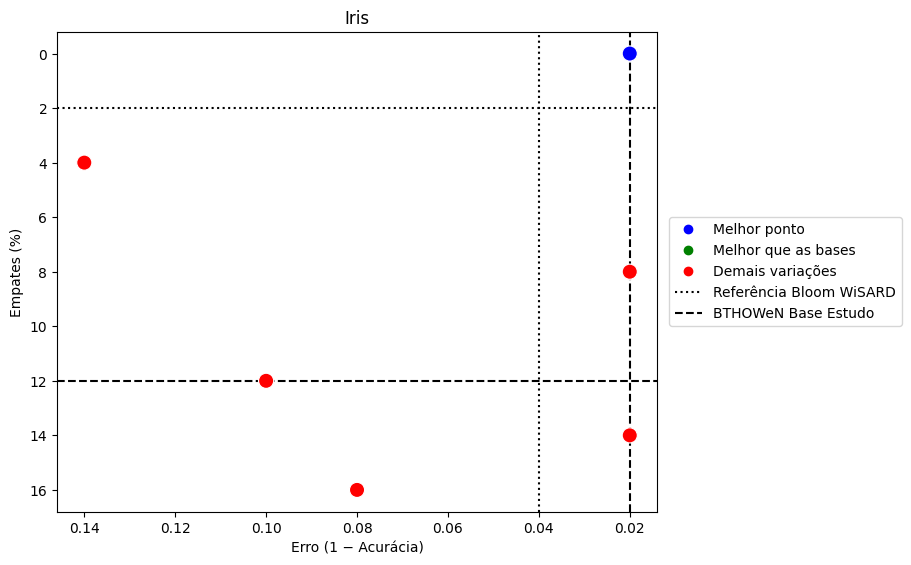
\includegraphics[width=1.1\textwidth]{figures/image1.png}
\caption{Relação entre erro e empates para o dataset Iris}
\label{fig:iris}
\end{figure}

\begin{figure}[H]
\centering
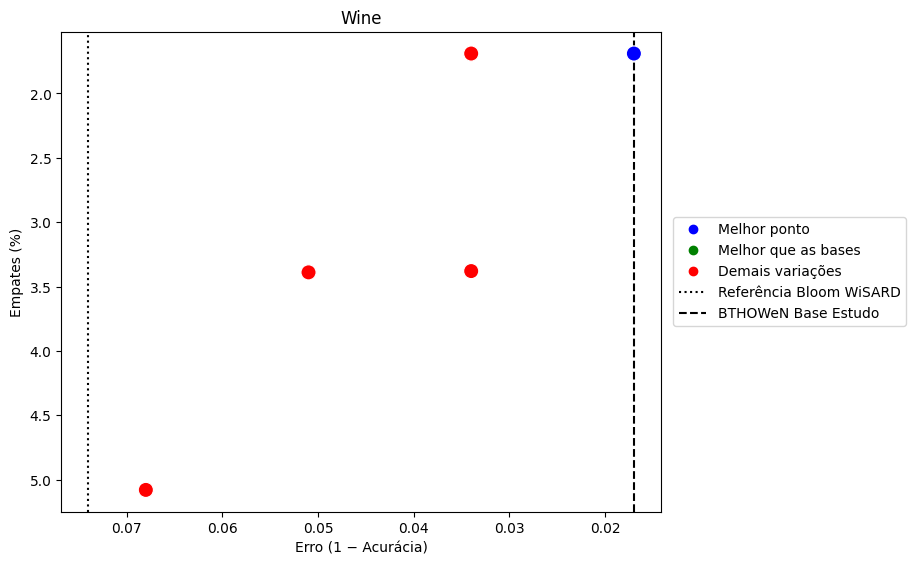
\includegraphics[width=1.1\textwidth]{figures/image3.png}
\caption{Relação entre erro e empates para o dataset Wine}
\label{fig:wine}
\end{figure}

\begin{figure}[H]
\centering
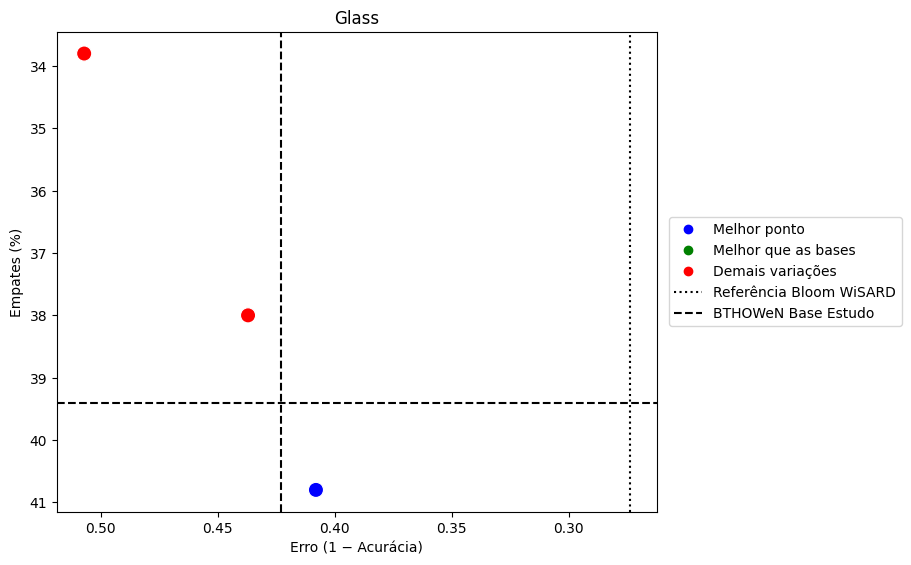
\includegraphics[width=1.1\textwidth]{figures/image5.png}
\caption{Relação entre erro e empates para o dataset Glass}
\label{fig:glass}
\end{figure}

\begin{figure}[H]
\centering
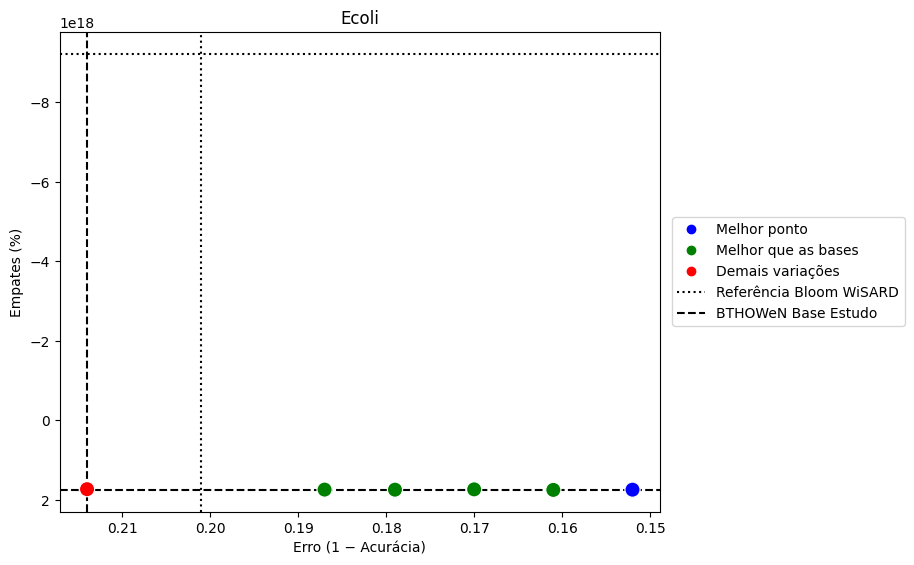
\includegraphics[width=1.1\textwidth]{figures/image6.png}
\caption{Relação entre erro e empates para o dataset Ecoli}
\label{fig:ecoli}
\end{figure}

\begin{figure}[H]
\centering
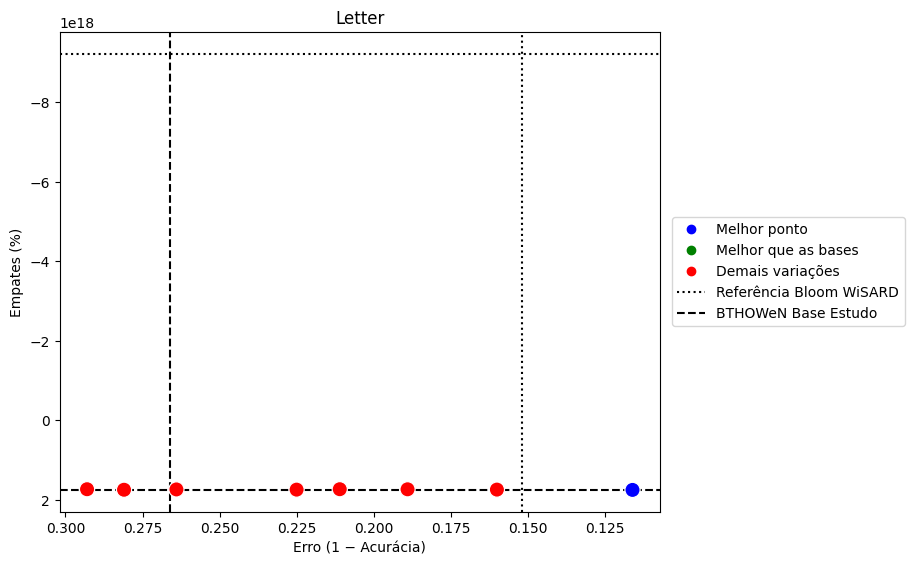
\includegraphics[width=1.1\textwidth]{figures/image12.png}
\caption{Relação entre erro e empates para o dataset Letter}
\label{fig:letter}
\end{figure}

\begin{figure}[H]
\centering
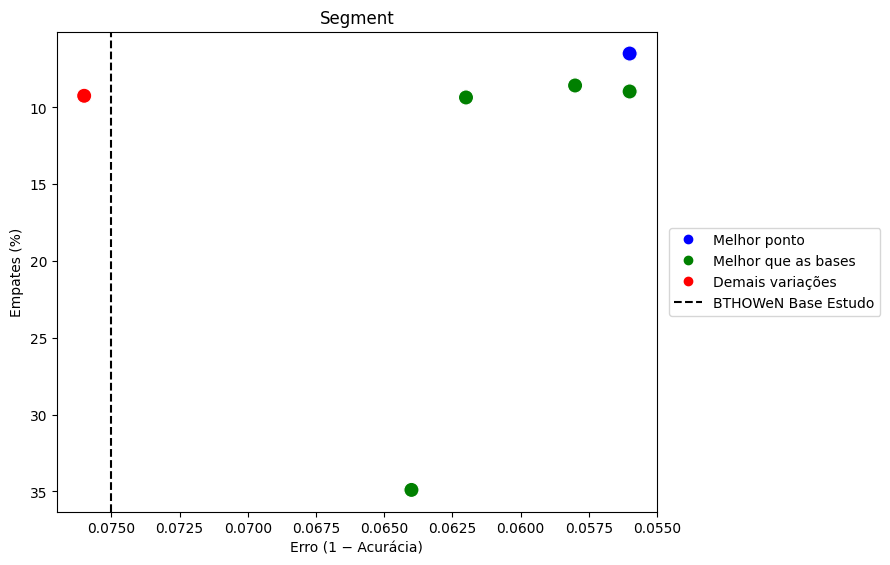
\includegraphics[width=1.1\textwidth]{figures/image2.png}
\caption{Relação entre erro e empates para o dataset Segment}
\label{fig:segment}
\end{figure}

\begin{figure}[H]
\centering
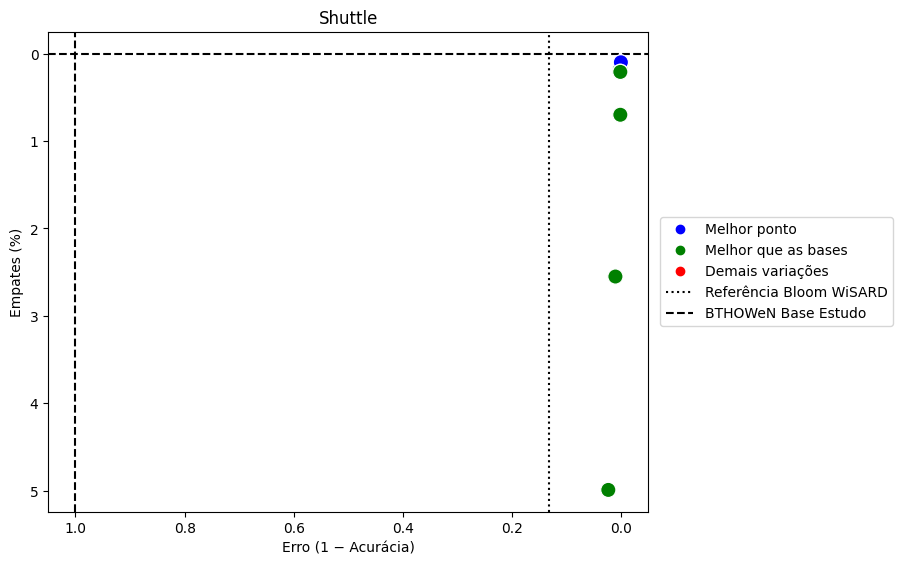
\includegraphics[width=1.1\textwidth]{figures/image9.png}
\caption{Relação entre erro e empates para o dataset Shuttle}
\label{fig:shuttle}
\end{figure}

\begin{figure}[H]
\centering
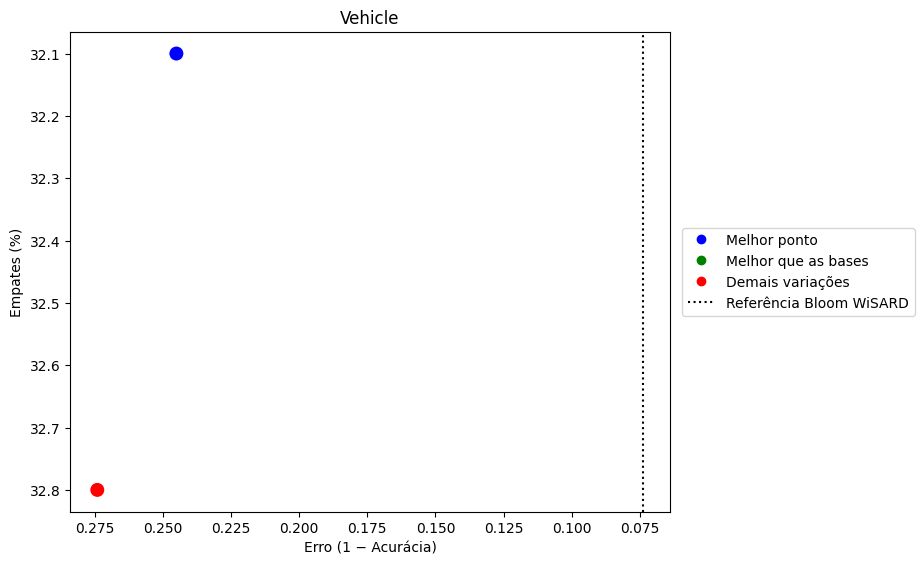
\includegraphics[width=1.1\textwidth]{figures/image7.png}
\caption{Relação entre erro e empates para o dataset Vehicle}
\label{fig:vehicle}
\end{figure}

\begin{figure}[H]
\centering
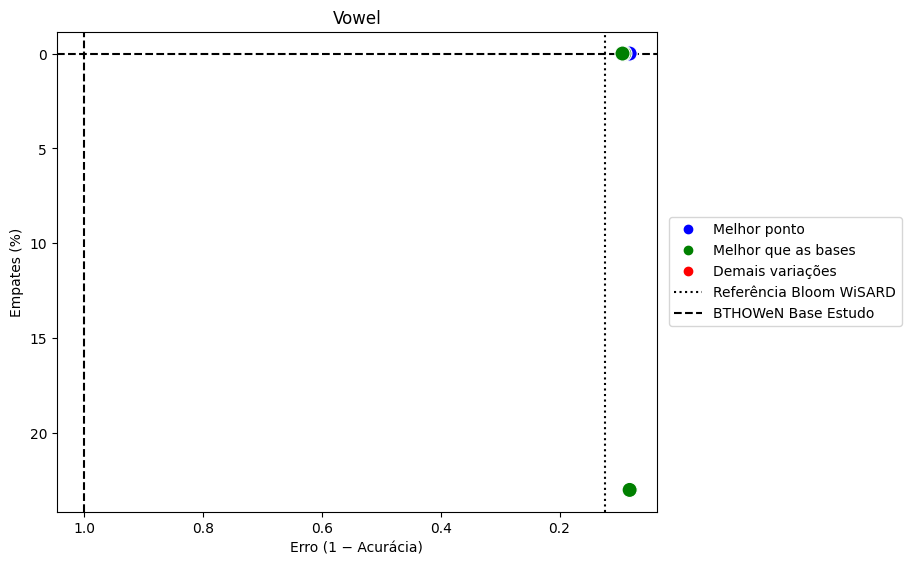
\includegraphics[width=1.1\textwidth]{figures/image8.png}
\caption{Relação entre erro e empates para o dataset Vowel}
\label{fig:vowel}
\end{figure}

\begin{figure}[H]
\centering
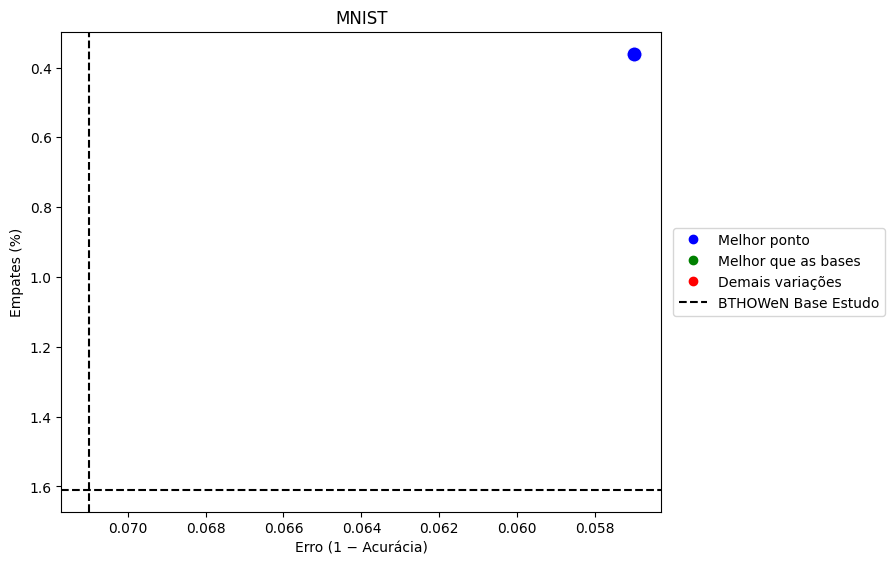
\includegraphics[width=1.1\textwidth]{figures/image11.png}
\caption{Relação entre erro e empates para o dataset MNIST}
\label{fig:mnist}
\end{figure}


\subsection{Resultados agregados}

Na tabela a seguir, apresentamos os parâmetros ótimos identificados para cada dataset, junto com as métricas de desempenho obtidas:

{\small
\begin{table}[H]
\caption{Parâmetros ótimos para cada dataset}
\renewcommand{\arraystretch}{1.1}
\begin{center}
\begin{tabular}{lccccccc}
\hline
\textbf{Dataset} & \textbf{b} & \textbf{OWeN} & \textbf{FE} & \textbf{FH} & \textbf{Melhor Bleaching} & \textbf{Execução} & \textbf{Empates (\%)} \\
\hline
Iris & 3 & \textcolor{blue}{2} & \textcolor{green}{256} & \textcolor{blue}{2} & 2 & \textcolor{red}{1} & \textcolor{red}{0} \\
Ecoli & \textcolor{red}{3} & \textcolor{green}{256} & \textcolor{green}{3} & 10 & \textcolor{red}{1} & 1 & \textcolor{green}{10.7} \\
Glass & \textcolor{green}{4} & \textcolor{green}{256} & \textcolor{green}{4} & \textcolor{green}{10} & 1 & 1 & \textcolor{red}{28.2} \\
Letter & \textcolor{green}{15} & \textcolor{green}{256} & \textcolor{green}{5} & \textcolor{green}{35} & \textcolor{red}{3} & 1 & \textcolor{red}{3.9} \\
Wine & \textcolor{green}{10} & 13 & \textcolor{green}{256} & \textcolor{green}{4} & 1 & -- & 1.7 \\
Segment & \textcolor{green}{10} & \textcolor{red}{18} & 1.14 & \textcolor{green}{3} & \textcolor{green}{2} & -- & 6.49 \\
Shuttle & \textcolor{green}{11} & \textcolor{red}{25} & 1.14 & \textcolor{green}{3} & \textcolor{red}{1} & -- & \textcolor{green}{0.1} \\
Vehicle & \textcolor{red}{15} & \textcolor{red}{12} & 256 & \textcolor{blue}{2} & 1 & -- & 20.2 \\
Vowel & \textcolor{red}{15} & \textcolor{red}{13} & \textcolor{green}{512} & \textcolor{green}{5} & 1 & -- & \textcolor{green}{24.4} \\
MNIST & \textcolor{green}{6} & \textcolor{green}{49} & \textcolor{green}{81.1} & \textcolor{green}{4} & -- & -- & -- \\
\hline
\end{tabular}
\end{center}
\end{table}
}

\section{Conclusão}

\ldots

\bibliographystyle{plain}
\bibliography{references}

\end{document}
